\documentclass[lang=cn,11pt,a4paper,cite=authornum]{paper}

\title{大数据技术基础 综合实验 \\ 实验报告}
\author{毛子恒 \\ 2019211397 \and 李康童 \\ 2019211408}
\institute{北京邮电大学\ 计算机学院}

\date{\zhtoday}

% 本文档命令
\nocite{*}

\begin{document}

\maketitle

\part{基础部分}

\section{概述}

\subsection{实验目的}

\begin{enumerate}
    \item 掌握Lambda架构
\end{enumerate}

\subsection{实验步骤}

\begin{enumerate}
    \item 安装kafka
    \item 安装Redis
    \item 运行推荐系统
\end{enumerate}

\section{实验结果及分析}

\paragraph{安装kafka}

安装并启动kafka的结果如\figref{fig:1}所示。

\begin{figure}[!htb]
    \centering
    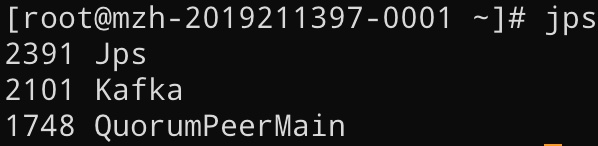
\includegraphics[width=0.5\textwidth]{./images/1.jpg}
    \caption{kafka启动结果\label{fig:1}}
\end{figure}

\paragraph{安装Redis}

安装并启动redis的结果如\figref{fig:2}所示。

\begin{figure}[!htb]
    \centering
    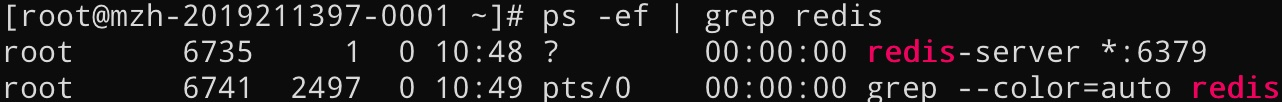
\includegraphics[width=\textwidth]{./images/2.jpg}
    \caption{redis启动结果\label{fig:2}}
\end{figure}

\paragraph{运行推荐系统}

步骤如下:

\begin{enumerate}
    \item 启动HDFS
    \item 启动zookeeper
    \item 启动HBase
    \item 配置HBase Thrift连接,以便python中的happybase库能够连接Hbase (详见 一些命令.txt)
    \item 在HBase中创建对应的表
    \item 启动load\_train\_ratings\_hbase.py(需要运行完)
    \item 启动redis
    \item 启动load\_movie\_redis.py(需要运行完)
    \item 启动Kafka 并创建 Kafka Topic
    \item 启动generatorRecord.py(这个程序会一直运行,不需要等待停止)
    \item 启动hbase2spark、kafkaStreaming、recommend
    \item 启动recommend\_server.py
    \item 启动recommend\_client.py
\end{enumerate}

推荐结果如\figref{fig:3}所示。

\begin{figure}[!htb]
    \centering
    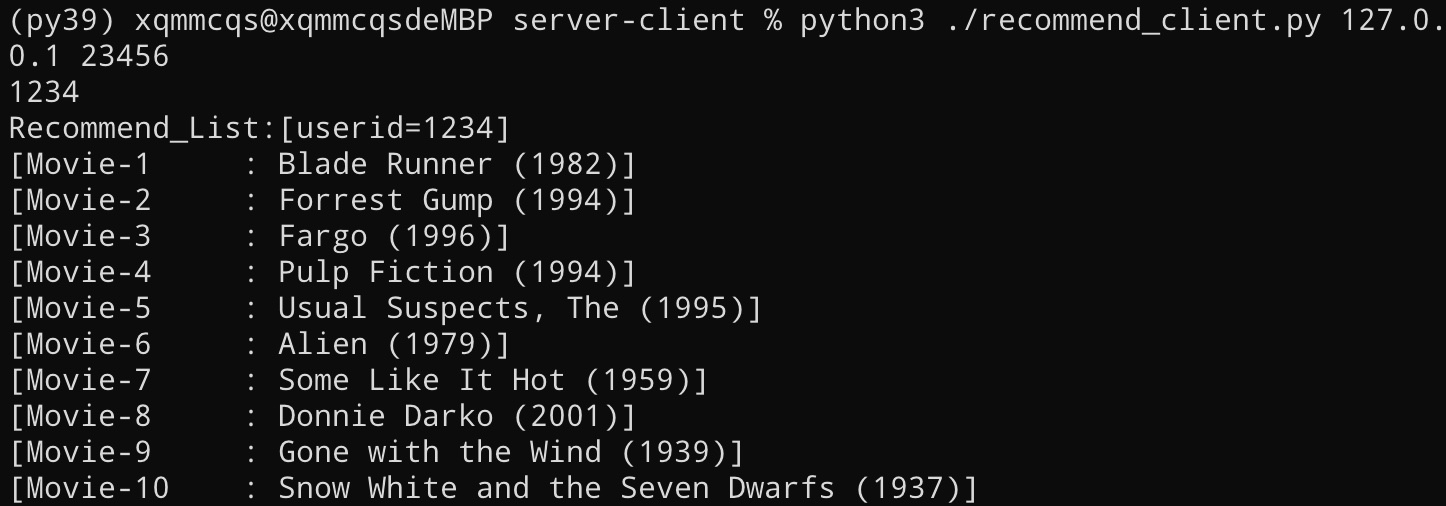
\includegraphics[width=\textwidth]{./images/3.jpg}
    \caption{推荐系统运行结果\label{fig:3}}
\end{figure}

\part{选做部分}

\subsection{实验步骤}

\begin{enumerate}
    \item 使用Hive/SparkSQL实现简易后台分析统计
    \item 将后台分析统计结果可视化
\end{enumerate}

\section{实验结果及分析}

\paragraph{启动Hive}

\begin{code}
\begin{minted}{shell}
hive --service hiveserver2 >/dev/null 2>&1 &
\end{minted}
\end{code}

\paragraph{创建表}

在Hive中创建外部表,连接到HBase的电影记录表。

\begin{code}
\begin{minted}{shell}
create external table movie_rating_details(
    key string,
    movieId int,
    rating int,
    times int,
    userId int)
    stored by
    'org.apache.hadoop.hive.hbase.HBaseStorageHandler'
    WITH SERDEPROPERTIES ("hbase.columns.mapping" =
    ":key,details:movieId,details:rating,details:timestamp,details:userId")
    TBLPROPERTIES("hbase.table.name" = "movie_records");
\end{minted}
\end{code}

创建表结果如\figref{fig:4}所示。

\begin{figure}[!htb]
    \centering
    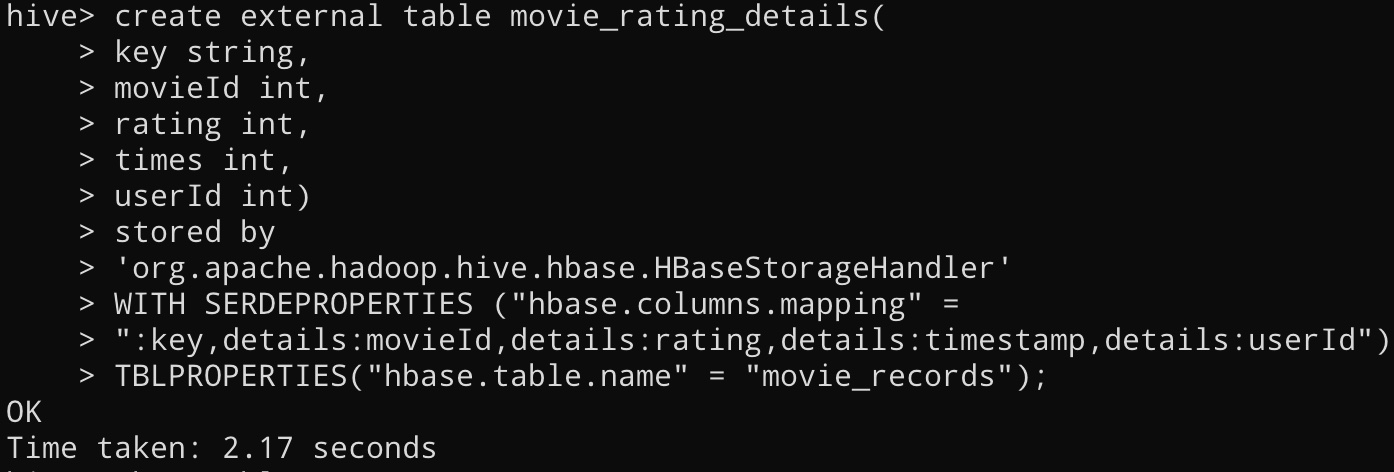
\includegraphics[width=\textwidth]{./images/4.jpg}
    \caption{Hive建表结果\label{fig:4}}
\end{figure}

表结构如\figref{fig:5}、\figref{fig:6}所示。

\begin{figure}[!htb]
    \centering
    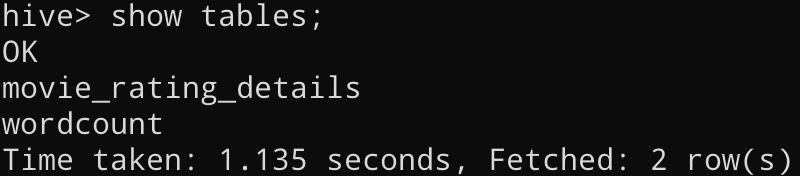
\includegraphics[width=0.6\textwidth]{./images/5.jpg}
    \caption{表名\label{fig:5}}
\end{figure}

\begin{figure}[!htb]
    \centering
    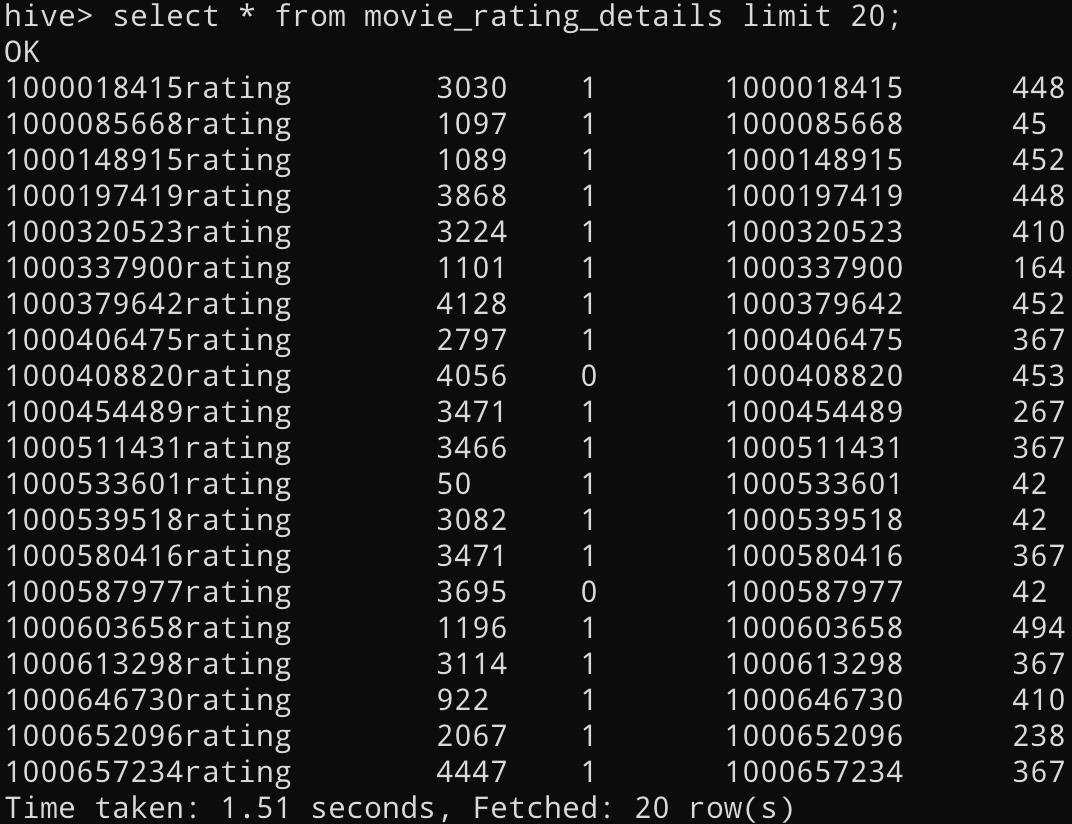
\includegraphics[width=0.8\textwidth]{./images/6.jpg}
    \caption{表内容\label{fig:6}}
\end{figure}

\paragraph{分析统计与可视化}

编写如下Python代码,实现分析统计功能。

\begin{code}
\begin{minted}{Python}
import sys
import time
from impala.dbapi import connect
import numpy as np
import pandas as pd
import matplotlib.pyplot as plt

def getArgs():
    argv = sys.argv[1:]
    return argv[0], argv[1], argv[2]

def load_file(filename):
    dataSet = pd.read_csv(filename)
    return dataSet

def hive_connect(host="mzh-2019211397-0001", port=10000):
    return connect(host=host, port=port, database='default')

if __name__ == '__main__':
    host, port, file_path = getArgs()
    conn = hive_connect(host, port)
    df = load_file(file_path)
    movieId2Category = dict()
    count_result = dict()
    for i in df.columns[4:]:
        count_result[i] = 0
    for row in df.iterrows():
        movieId2Category[row[1]['movieId']] = row[1][4:].to_list()
    plt.ion()
    ax = df.columns[4:].to_list()
    while True:
        count_result = [0] * 19
        time.sleep(1800)
        with conn.cursor() as cursor:
            cursor.execute('SELECT movieId, count(*) FROM movie_rating_details GROUP BY movieId')
            for row in cursor:
                for i, value in enumerate(movieId2Category[row[0]]):
                    count_result[i] += value * row[1]
        print(count_result)
        plt.clf()
        plt.bar(ax,count_result) 
        plt.xticks(rotation=90)
        plt.pause(0.001)
\end{minted}
\end{code}

代码从Hive中读取电影的记录,并且根据movies.csv中的电影类别信息统计不同类型的电影数目,最后采用matplotlib进行可视化,程序每隔半个小时更新图表。

采用以下命令运行:

\begin{code}
\begin{minted}{shell}
    python3 category_count.py mzh-2019211397-0001 10000 "../data/movies.csv"
\end{minted}
\end{code}

运行结果如\figref{fig:7}所示。

\begin{figure}[!htb]
    \centering
    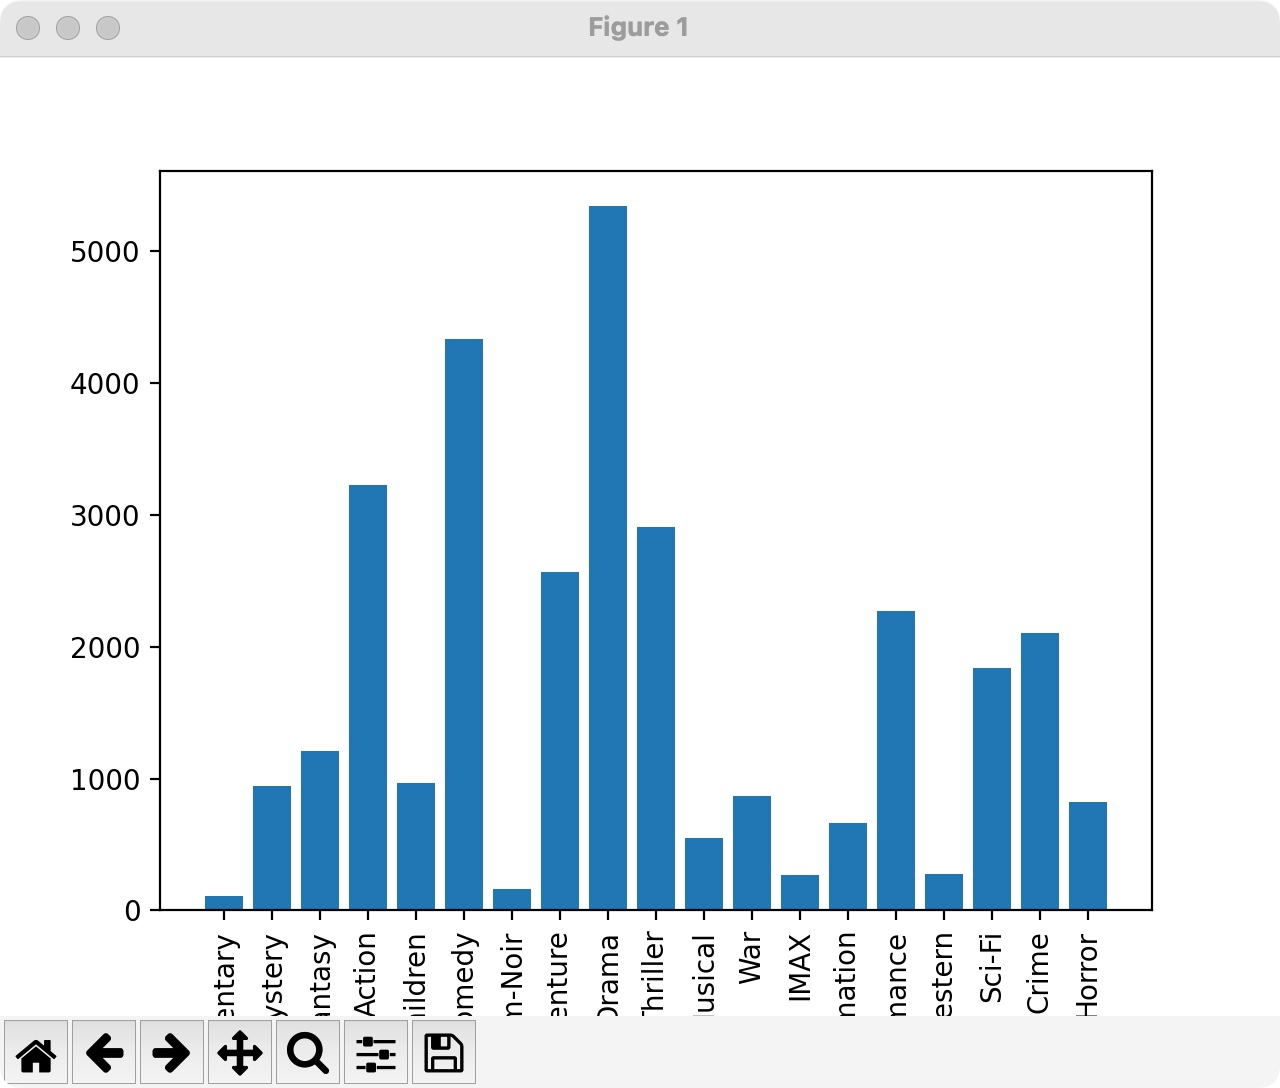
\includegraphics[width=0.8\textwidth]{./images/7.jpg}
    \caption{电影类别统计\label{fig:7}}
\end{figure}

\part{提高部分}

见\ref{survey}节。

\section{实验总结}

本次实验中我们基于Lambda架构搭建起简单的推荐系统,并且实现了简单的后台监控功能。在实验过程中我们对Lambda架构、HBase、Spark Streaming组件的理解更加深刻。

\newpage

\appendix

\section{大数据框架调研}

\label{survey}

\end{document}
